\documentclass[onecolumn,letterpaper,11pt]{article}

%===================================================================
%===================================================================
% Include common packages, environments, counters etc

\usepackage{bbm}       % Blackboard style cm fonts
\usepackage{here}      % Emulation of obsolete package for ``here'' floats
\usepackage{xcolor}    % Driver independent color extensions
\usepackage{amsfonts}  % TEX fonts from American Mathematical Society
\usepackage{cite}      % Improved citation handling
\usepackage{url}       % Verbatim with URL-sensitive line breaks
\usepackage{verbatim}  % Reimplementation of and extensions to LATEX verbatim
\usepackage{fancyvrb}  % Sophisticated verbatim text
\usepackage{microtype} % For better formatting to take advantage of pdflatex
\usepackage{graphicx}  % For better formatting to take advantage of pdflatex
\usepackage{longtable} % For listing config parameters
\usepackage{hyperref}  % Enable links in bibtex urls
\usepackage[footnotesize]{caption}
\hypersetup{
    colorlinks = true,
    urlcolor = {blue},
    linkcolor = {blue},
}

%============================================================
% Algorithm environment header:
%   This environment is used to "wrap" the algorithmic
%   environment. If we do the typcial thing which is to wrap
%   an algorithmic block inside the "algorithm" environment, 
%   the whole algorithm will not page-break. But not wrapping
%   it loses the header. This environment fakes the algorithm
%   header and leaves the algorithmic block unwrapped so the 
%   net effect is that the algorithm will automatically split
%   across multiple pages.
% To return to a non-page-break version, replace with:
% \begin{algorithm}
% \caption{My caption}
% body
% \end{algorithm}
%============================================================
\newcounter{myalgctr}
\setcounter{myalgctr}{0}

%============================================================
% Begin: the mbalg environment: A wrapper to the algorithmic
%        environment that allows split over page breaks.
%============================================================
\newenvironment{mbalg}[1]{
\noindent 
\rule{\textwidth}{1pt}

\vspace{-0.04in}
\refstepcounter{algorithm}
\noindent
{\bf Algorithm \arabic{algorithm}:} #1

\vspace{-0.125in}
\noindent
\rule{\textwidth}{0.6pt} 

}{\vspace{-0.125in}

\noindent
\rule{\textwidth}{0.6pt}
}
%============================================================


%============================================================
% Begin: Local color definitions
%============================================================
\definecolor{mbeige}{rgb}{0.875,0.859,0.765}
\definecolor{param-blue}{rgb}{0.1,0.1,0.765}
\definecolor{mygrey}{rgb}{0.94,0.94,0.94}
\definecolor{menublue}{rgb}{0.22,0.38,0.71}
\definecolor{menugreen}{rgb}{0,0.6,0}
\definecolor{myorange}{rgb}{1,0.65,0.35}
\definecolor{bhvcolor}{rgb}{0.73,0.35,0.18}
\definecolor{magenta}{rgb}{0.8,0,0.8}
\definecolor{empty}{rgb}{0.5,0.5,0.5} 
\definecolor{invisible}{rgb}{0.5,0.5,0.5} 
\definecolor{yellow}{rgb}{1.000,1.000,0.000} 
\definecolor{purple}{rgb}{0.502,0.000,0.502} 
\definecolor{brown}{rgb}{0.647,0.165,0.165} 
\definecolor{black}{rgb}{0.000,0.000,0.000} 
\definecolor{blue}{rgb}{0.000,0.000,1.000} 
\definecolor{red}{rgb}{1.000,0.000,0.000} 
\definecolor{yellow}{rgb}{1.000,1.000,0.000} 
\definecolor{white}{rgb}{1.000,1.000,1.000} 
\definecolor{darkgreen}{rgb}{0.000,0.392,0.000} 
\definecolor{darkolivegreen}{rgb}{0.333,0.420,0.184} 
\definecolor{darkred}{rgb}{0.545,0.000,0.000} 
\definecolor{green}{rgb}{0.000,0.502,0.000} 
\definecolor{macbeige}{rgb}{0.875,0.859,0.765} 
\definecolor{macpurple}{rgb}{0.286,0.239,0.471} 
\definecolor{antiquewhite}{rgb}{0.980,0.922,0.843} 
\definecolor{aqua}{rgb}{0.000,1.000,1.000} 
\definecolor{aquamarine}{rgb}{0.498,1.000,0.831} 
\definecolor{azure}{rgb}{0.941,1.000,1.000} 
\definecolor{beige}{rgb}{0.961,0.961,0.863} 
\definecolor{bisque}{rgb}{1.000,0.894,0.769} 
\definecolor{blanchedalmond}{rgb}{1.000,0.922,0.804} 
\definecolor{blueviolet}{rgb}{0.541,0.169,0.886} 
\definecolor{brown}{rgb}{0.647,0.165,0.165} 
\definecolor{burlywood}{rgb}{0.871,0.722,0.529} 
\definecolor{cadetblue}{rgb}{0.373,0.620,0.627} 
\definecolor{chartreuse}{rgb}{0.498,1.000,0.000} 
\definecolor{chocolate}{rgb}{0.824,0.412,0.118} 
\definecolor{coral}{rgb}{1.000,0.498,0.314} 
\definecolor{cornsilk}{rgb}{1.000,0.973,0.863} 
\definecolor{cornflowerblue}{rgb}{0.392,0.584,0.929} 
\definecolor{crimson}{rgb}{0.871,0.078,0.235} 
\definecolor{cyan}{rgb}{0.000,1.000,1.000} 
\definecolor{darkblue}{rgb}{0.000,0.000,0.545} 
\definecolor{darkcyan}{rgb}{0.000,0.545,0.545} 
\definecolor{darkgoldenrod}{rgb}{0.722,0.525,0.043} 
\definecolor{darkgray}{rgb}{0.663,0.663,0.663} 
\definecolor{darkkhaki}{rgb}{0.741,0.718,0.420} 
\definecolor{darkmagenta}{rgb}{0.545,0.000,0.545} 
\definecolor{darkorange}{rgb}{1.000,0.549,0.000} 
\definecolor{darkorchid}{rgb}{0.600,0.196,0.800} 
\definecolor{darksalmon}{rgb}{0.914,0.588,0.478} 
\definecolor{darkseagreen}{rgb}{0.561,0.737,0.561} 
\definecolor{darkslateblue}{rgb}{0.282,0.239,0.545} 
\definecolor{darkslategray}{rgb}{0.184,0.310,0.310} 
\definecolor{darkturquoise}{rgb}{0.000,0.808,0.820} 
\definecolor{darkviolet}{rgb}{0.580,0.000,0.827} 
\definecolor{deeppink}{rgb}{1.000,0.078,0.576} 
\definecolor{deepskyblue}{rgb}{0.000,0.749,1.000} 
\definecolor{dimgray}{rgb}{0.412,0.412,0.412} 
\definecolor{dodgerblue}{rgb}{0.118,0.565,1.000} 
\definecolor{firebrick}{rgb}{0.698,0.133,0.133} 
\definecolor{floralwhite}{rgb}{1.000,0.980,0.941} 
\definecolor{forestgreen}{rgb}{0.133,0.545,0.133} 
\definecolor{fuchsia}{rgb}{1.000,0.000,1.000} 
\definecolor{gainsboro}{rgb}{0.863,0.863,0.863} 
\definecolor{ghostwhite}{rgb}{0.973,0.973,1.000} 
\definecolor{gold}{rgb}{1.000,0.843,0.000} 
\definecolor{goldenrod}{rgb}{0.855,0.647,0.125} 
\definecolor{greenyellow}{rgb}{0.678,1.000,0.184} 
\definecolor{honeydew}{rgb}{0.941,1.000,0.941} 
\definecolor{hotpink}{rgb}{1.000,0.412,0.706} 
\definecolor{indianred}{rgb}{0.804,0.361,0.361} 
\definecolor{indigo}{rgb}{0.294,0.000,0.510} 
\definecolor{ivory}{rgb}{1.000,1.000,0.941} 
\definecolor{khaki}{rgb}{0.941,0.902,0.549} 
\definecolor{lavender}{rgb}{0.902,0.902,0.980} 
\definecolor{lavenderblush}{rgb}{1.000,0.941,0.961} 
\definecolor{lawngreen}{rgb}{0.486,0.988,0.000} 
\definecolor{lemonchiffon}{rgb}{1.000,0.980,0.804} 
\definecolor{lightblue}{rgb}{0.678,0.847,0.902} 
\definecolor{lightcoral}{rgb}{0.941,0.502,0.502} 
\definecolor{lightcyan}{rgb}{0.878,1.000,1.000} 
\definecolor{lightgoldenrod}{rgb}{0.980,0.980,0.824} 
\definecolor{lightgray}{rgb}{0.827,0.827,0.827} 
\definecolor{lightgreen}{rgb}{0.565,0.933,0.565} 
\definecolor{lightpink}{rgb}{1.000,0.714,0.757} 
\definecolor{lightsalmon}{rgb}{1.000,0.627,0.478} 
\definecolor{lightseagreen}{rgb}{0.125,0.698,0.667} 
\definecolor{lightskyblue}{rgb}{0.529,0.808,0.980} 
\definecolor{lightslategray}{rgb}{0.467,0.533,0.600} 
\definecolor{lightsteelblue}{rgb}{0.690,0.769,0.871} 
\definecolor{lightyellow}{rgb}{1.000,1.000,0.878} 
\definecolor{lime}{rgb}{0.000,1.000,0.000} 
\definecolor{limegreen}{rgb}{0.196,0.804,0.196} 
\definecolor{linen}{rgb}{0.980,0.941,0.902} 
%\definecolor{magenta}{rgb}{1.000,0.000,1.000} 
\definecolor{maroon}{rgb}{0.502,0.000,0.000} 
\definecolor{mediumblue}{rgb}{0.000,0.000,0.804} 
\definecolor{mediumprchid}{rgb}{0.729,0.333,0.827} 
\definecolor{mediumseagreen}{rgb}{0.235,0.702,0.443} 
\definecolor{mediumslateblue}{rgb}{0.482,0.408,0.933} 
\definecolor{mediumspringgreen}{rgb}{0.000,0.980,0.604} 
\definecolor{mediumturquoise}{rgb}{0.282,0.820,0.800} 
\definecolor{mediumvioletred}{rgb}{0.780,0.082,0.522} 
\definecolor{midnightblue}{rgb}{0.098,0.098,0.439} 
\definecolor{mintcream}{rgb}{0.961,1.000,0.980} 
\definecolor{mistyrose}{rgb}{1.000,0.894,0.882} 
\definecolor{moccasin}{rgb}{1.000,0.894,0.710} 
\definecolor{navajowhite}{rgb}{1.000,0.871,0.678} 
\definecolor{navy}{rgb}{0.000,0.000,0.502} 
\definecolor{oldlace}{rgb}{0.992,0.961,0.902} 
\definecolor{olive}{rgb}{0.502,0.502,0.000} 
\definecolor{olivedrab}{rgb}{0.420,0.557,0.137} 
\definecolor{orange}{rgb}{1.000,0.647,0.000} 
\definecolor{orangered}{rgb}{1.000,0.271,0.000} 
\definecolor{orchid}{rgb}{0.855,0.439,0.839} 
\definecolor{oxfordindigo}{rgb}{0.255,0.341,0.596} 
\definecolor{palegreen}{rgb}{0.596,0.984,0.596} 
\definecolor{paleturquoise}{rgb}{0.686,0.933,0.933} 
\definecolor{palevioletred}{rgb}{0.859,0.439,0.576} 
\definecolor{papayawhip}{rgb}{1.000,0.937,0.835} 
\definecolor{peachpuff}{rgb}{1.000,0.855,0.725} 
\definecolor{pelegoldenrod}{rgb}{0.933,0.910,0.667} 
\definecolor{peru}{rgb}{0.804,0.522,0.247} 
\definecolor{pink}{rgb}{1.000,0.753,0.796} 
\definecolor{plum}{rgb}{0.867,0.627,0.867} 
\definecolor{powderblue}{rgb}{0.690,0.878,0.902} 
\definecolor{purple}{rgb}{0.502,0.000,0.502} 
\definecolor{rosybrown}{rgb}{0.737,0.561,0.561} 
\definecolor{royalblue}{rgb}{0.255,0.412,0.882} 
\definecolor{saddlebrowm}{rgb}{0.545,0.271,0.075} 
\definecolor{salmon}{rgb}{0.980,0.502,0.447} 
\definecolor{sandybrown}{rgb}{0.957,0.643,0.376} 
\definecolor{seagreen}{rgb}{0.180,0.545,0.341} 
\definecolor{seashell}{rgb}{1.000,0.961,0.933} 
\definecolor{sienna}{rgb}{0.627,0.322,0.176} 
\definecolor{silver}{rgb}{0.753,0.753,0.753} 
\definecolor{skyblue}{rgb}{0.529,0.808,0.922} 
\definecolor{slateblue}{rgb}{0.416,0.353,0.804} 
\definecolor{slategray}{rgb}{0.439,0.502,0.565} 
\definecolor{snow}{rgb}{1.000,0.980,0.980} 
\definecolor{springgreen}{rgb}{0.000,1.000,0.498} 
\definecolor{steelblue}{rgb}{0.275,0.510,0.706} 
\definecolor{tan}{rgb}{0.824,0.706,0.549} 
\definecolor{teal}{rgb}{0.000,0.502,0.502} 
\definecolor{thistle}{rgb}{0.847,0.749,0.847} 
\definecolor{tomatao}{rgb}{1.000,0.388,0.278} 
\definecolor{turquoise}{rgb}{0.251,0.878,0.816} 
\definecolor{violet}{rgb}{0.933,0.510,0.933} 
\definecolor{wheat}{rgb}{0.961,0.871,0.702} 
\definecolor{whitesmoke}{rgb}{0.961,0.961,0.961} 
\definecolor{yellowgreen}{rgb}{0.604,0.804,0.196} 
\definecolor{lightmenublue}{rgb}{0.52,0.68,0.91} 
\definecolor{gray99}{rgb}{0.99,0.99,0.99}  
\definecolor{gray98}{rgb}{0.98,0.98,0.98}  
\definecolor{gray97}{rgb}{0.97,0.97,0.97}  
\definecolor{gray96}{rgb}{0.96,0.96,0.96}  
\definecolor{gray94}{rgb}{0.94,0.94,0.94}  
\definecolor{gray93}{rgb}{0.93,0.93,0.93}  
\definecolor{gray92}{rgb}{0.92,0.92,0.92}  
\definecolor{gray91}{rgb}{0.91,0.91,0.91}  
\definecolor{gray05}{rgb}{0.050,0.050,0.050} 
\definecolor{gray10}{rgb}{0.100,0.100,0.100} 
\definecolor{gray15}{rgb}{0.150,0.150,0.150} 
\definecolor{gray20}{rgb}{0.200,0.200,0.200} 
\definecolor{gray25}{rgb}{0.250,0.250,0.250} 
\definecolor{gray30}{rgb}{0.300,0.300,0.300} 
\definecolor{gray35}{rgb}{0.350,0.350,0.350} 
\definecolor{gray40}{rgb}{0.400,0.400,0.400} 
\definecolor{gray45}{rgb}{0.450,0.450,0.450} 
\definecolor{gray50}{rgb}{0.500,0.500,0.500} 
\definecolor{gray55}{rgb}{0.550,0.550,0.550} 
\definecolor{gray60}{rgb}{0.600,0.600,0.600} 
\definecolor{gray65}{rgb}{0.650,0.650,0.650} 
\definecolor{gray70}{rgb}{0.700,0.700,0.700} 
\definecolor{gray75}{rgb}{0.750,0.750,0.750} 
\definecolor{gray80}{rgb}{0.800,0.800,0.800} 
\definecolor{gray85}{rgb}{0.850,0.850,0.850} 
\definecolor{gray90}{rgb}{0.900,0.900,0.900} 
\definecolor{gray95}{rgb}{0.950,0.950,0.950} 

%==================================================
\newlength{\pin}
\setlength{\pin}{0.2in}

\newenvironment{hangpar}[1]{\list{}{
    \setlength{\listparindent}{1.5em}       \setlength{\itemindent}{0pt}
    \setlength{\itemsep}{0pt}               \setlength{\parindent}{0pt}
    \setlength{\rightmargin}{0pt}           \setlength{\leftmargin}{#1}
               \parsep                                 \medskipamount}%
    \item\hspace{-\leftmargin}\noindent\ignorespaces}
    {\endlist}


%==================================================
% Name the current release
\newcommand{\release}{15.5.1}

%==================================================
% Name the current release
\newcommand{\moosivp}{MOOS-IvP}
\newcommand{\moosdb}{MOOSDB}
\newcommand{\moos}{MOOS}
\newcommand{\helm}{Helm}

%==================================================
% A few of our own counters defined
\newcounter{alisting}
\newcounter{exercise}
\newcounter{slisting}
\newcounter{listing}
\newcounter{tip}
\newcounter{expnum}
\newcounter{exnum}

%==================================================
% Hazard Search Macros
\newcommand{\pd}{{P_{_D}}}
\newcommand{\pc}{{P_{_C}}}
\newcommand{\pfa}{P_{_{FA}}}

%==================================================
% IvPBuild Toolbox Macros 
\newcommand{\summit}{\var{summit}}
\newcommand{\sdelta}{\var{summitdelta}}
\newcommand{\pwid}{\var{peakwidth}}
\newcommand{\bwid}{\var{basewidth}}
\newcommand{\minu}{\var{minutil}}
\newcommand{\maxu}{\var{maxutil}}
\newcommand{\sumi}{\var{summitinsist}}
\newcommand{\vwrap}{\var{valuewrap}}
\newcommand{\zpeak}{\var{ZAIC\_PEAK}}
\newcommand{\zvec}{\var{ZAIC\_Vector}}
\newcommand{\zleq}{\var{ZAIC\_LEQ}}
\newcommand{\zheq}{\var{ZAIC\_HEQ}}

\newcommand{\blankpage}{\clearpage \hspace{0.1in} \newpage}
\newcommand{\pskip}{\vspace{4pt}}
\newcommand{\prevblue}[1][0.07in]{\vspace{#1}  \small \color{menublue}}
\newcommand{\prevgreen}[1][0.07in]{\vspace{#1} \small \color{menugreen}}
\newcommand{\prevbhv}[1][0.07in]{\vspace{#1}   \small \color{bhvcolor}}
\newcommand{\postverb}[1][0.07in]{\vspace{#1} \normalsize \color{black}}

\newcommand{\myurl}[1]{\textcolor{menublue}{\url{#1}}}
\newcommand{\urlx}[1]{\textcolor{menublue}{\url{#1}}}

\newcommand{\noop}[1]{}
\newcommand{\fullcite}[1]{\bibentry{#1}.}
\newcommand{\doc}[1]{}
%\newcommand{\urlxx}[2]{\noindent \textcolor{menublue}{\url{#1}} \noop{#2}}
\newcommand{\urlxx}[2]{\noindent \textcolor{menublue}{\url{#1}}}


%\newcommand{\urlxx}[2]{\vspace{0.12in} \noindent 
%\textcolor{menublue}{\url{#1}} \noop{#2}\vspace{0.12in}}

%=======================================================
% special formatting for MOOS parameters
%=======================================================
% default size
\newcommand{\pvar}[1]{\textcolor{menublue}{\small \bf \tt #1}}
\newcommand{\pivar}[1]{\textcolor{menublue}{\small \tt #1}}
\newcommand{\psvar}[1]{\textcolor{menublue}{\small \tt #1}}

% bit bigger
\newcommand{\psvvar}[1]{\textcolor{menublue}{\footnotesize \tt #1}}
\newcommand{\pvvar}[1]{\textcolor{menublue}{\footnotesize \tt #1}}

% bit bigger
\newcommand{\psvarr}[1]{\textcolor{menublue}{\tt #1}}
\newcommand{\pvarr}[1]{\textcolor{menublue}{\tt #1}}

%=======================================================
% special formatting for Behavior parameters
%=======================================================
% default size
\newcommand{\bvar}[1]{\textcolor{bhvcolor}{\small \bf \tt #1}}
\newcommand{\bivar}[1]{\textcolor{bhvcolor}{\small \tt #1}}
\newcommand{\bsvar}[1]{\textcolor{bhvcolor}{\small \tt #1}}
% bit bigger
\newcommand{\bsvvar}[1]{\textcolor{bhvcolor}{\footnotesize \tt #1}}
\newcommand{\bvvar}[1]{\textcolor{bhvcolor}{\footnotesize \tt #1}}
% bit bigger
\newcommand{\bsvarr}[1]{\textcolor{bhvcolor}{\tt #1}}
\newcommand{\bvarr}[1]{\textcolor{bhvcolor}{\tt #1}}

%=======================================================
% special formatting for MOOS variables
%=======================================================
\newcommand{\wvar}[1]{\textcolor{white}{\small \tt #1}}
\newcommand{\mvar}[1]{\textcolor{menugreen}{\small \tt #1}}
\newcommand{\mivar}[1]{\textcolor{menugreen}{\small \tt #1}}
\newcommand{\msvar}[1]{\textcolor{menugreen}{\small \tt #1}}

% bit smaller
\newcommand{\mvvar}[1]{\textcolor{menugreen}{\footnotesize \tt #1}}
\newcommand{\msvvar}[1]{\textcolor{menugreen}{\footnotesize \tt #1}}

% bit bigger
\newcommand{\mvarr}[1]{\textcolor{menugreen}{\tt #1}}
\newcommand{\msvarr}[1]{\textcolor{menugreen}{\tt #1}}


%=======================================================
% special formatting for command-line commands
%=======================================================
\newcommand{\cmd}[1]{{\textcolor{magenta}{\small \tt #1}}}

%=======================================================
% special formatting for MOOS applications
%=======================================================
\newcommand{\app}[1]{{\textcolor{magenta}{\small \tt #1}}}
\newcommand{\aapp}[1]{{\textcolor{magenta}{\footnotesize \tt #1}}}

%=======================================================
% special formatting for variables in general
%=======================================================
\newcommand{\var}[1]{{\small \tt #1}}
\newcommand{\varr}[1]{{\tt #1}}
\newcommand{\vvar}[1]{{\footnotesize \tt #1}}

%=======================================================
% special formatting for functions
%=======================================================
\newcommand{\func}[1] {\textcolor{myorange}{\small \tt #1}}
\newcommand{\funcc}[1]{{\tt #1}}
\newcommand{\ffunc}[1]{{\footnotesize \tt #1}}

%=======================================================
% special formatting for verbatim inside math
%=======================================================
\newcommand{\hvar}[1]{\mbox{{\small \tt #1}}}
\newcommand{\hvvar}[1]{\mbox{{\footnotesize \tt #1}}}
\newcommand{\hvvvar}[1]{\mbox{{\tiny \tt #1}}}

%=======================================================
% Purposeful no-ops used only by latex-to-wiki translation
%=======================================================
\newcommand{\wikilink}[1]{}
\newcommand{\wikidoc}[1]{}
\newcommand{\wikisec}[1]{\setcounter{listing}{0}}
\newcommand{\wikihint}[1]{}
\newcommand{\wikitablehint}[1]{}
\newcommand{\wikiMathLarge}{}
\newcommand{\wikispace}{}
\newcommand{\wikiMathLARGE}{}
\newcommand{\wikiMathlarge}{}
\newcommand{\wikisub}{}
\newcommand{\wikinoref}{}
\newcommand{\helplevelsec}{}
\newcommand{\helplevelsubsec}{}
\newcommand{\helpsection}{\section*}
\newcommand{\helpsubsection}{\subsection*}

%\newcommand{\urlyoutube}[1]{\raggedright \url{#1}}
\newcommand{\urlvideo}[2]{\raggedright {\textcolor{menublue} {\tt video:(#2):}} \url{#1}}

%=======================================================
% Support for lab cover pages
\newcommand{\labtitle}[1]{ \huge #1 \normalsize \\}
\newcommand{\labsubtitle}[1]{#1 \\}
\newcommand{\labcourse}[1]{ \large #1 \normalsize \\}
\newcommand{\labdate}[1]{ \large {\bf #1} \normalsize \\}
\newcommand{\labauth}[1]{ #1 \\}
\newcommand{\labtocdepth}[1]{}
\newcommand{\labpng}[2]{\includegraphics[width=#1\textwidth]{#2} \\}
\newcommand{\labline}{\noindent \textcolor{gray70}{\rule{1.0\textwidth}{0.1pt}}}

\newcommand{\labtoc}[1]{
   \renewcommand\contentsname{}
   \labline
   \vspace{-0.7in}
   \begin{#1}
   \tableofcontents
   \end{#1}
   \labline}

\newenvironment{labcover}{\begin{center}}{\end{center}} 
\newenvironment{labinfo}{}{} 

\newcommand{\labinfoheader}[1]{\noindent #1}

\newcommand{\styletip}[1]{\subsubsection*{\refstepcounter{tip}\textcolor{menublue}
{Style Tip \#\arabic{tip} #1}}}%


%=======================================================
\newenvironment{packed_itemize}[1][1]{
\begin{itemize}
  \setlength{\itemsep}{#1pt}
  \setlength{\parskip}{0pt}
  \setlength{\parsep}{0pt}
}{\end{itemize}}

\newenvironment{packed_enumerate}[1][1]{
\begin{enumerate}
  \setlength{\itemsep}{#1pt}
  \setlength{\parskip}{0pt}
  \setlength{\parsep}{0pt}
}{\end{enumerate}}

% Basic listing environment, includes section number
\newenvironment{bentry}[1]{
\begin{itemize}
\item  \textcolor{menublue}{\bibentry{#1}.} \newline
\noindent
}{\end{itemize}}

% Basic listing environment, includes section number
\newenvironment{listing}[1]{
  \refstepcounter{listing}
  \noindent
  {\em Listing \thesection.\arabic{listing}: #1.} \noindent}

% Same listing environment but does not include section number
\newenvironment{listingx}[1]{
  \refstepcounter{listing}
  \noindent
  {\em Listing \arabic{listing}: #1.} \noindent}

\newenvironment{consoleverb}{\SaveVerbatim{SVerbEnv}}
  {\endSaveVerbatim%
  \vspace{0.1in}%
  \noindent% 
  \fcolorbox{black}{mygrey}{\makebox[0.95\textwidth][l]
  {\footnotesize\BUseVerbatim{SVerbEnv}}% 
  \normalsize}%
  \vspace{0.1in}}

\newenvironment{cstyle}[1]{
  \vspace{0.1in}%
  \noindent% 
  \fcolorbox{black}{mygrey}{\makebox[0.95\textwidth][l]
  {#1}}%
  \vspace{0.1in}}

\newenvironment{fileverb}{\SaveVerbatim{SVerbEnv}}
  {\endSaveVerbatim%
  \vspace{0.1in}%
  \noindent%
  \fcolorbox{black}{mbeige}{\makebox[0.95\textwidth][l]
  {\footnotesize\BUseVerbatim{SVerbEnv}}%
  \normalsize}%
  \vspace{0.1in}}

\newenvironment{fileverbs}{\SaveVerbatim{SVerbEnv}}
  {\endSaveVerbatim%
  \vspace{0.1in}%
  \noindent%
  \fcolorbox{black}{mbeige}{\makebox[0.95\textwidth][l]
  {\scriptsize\BUseVerbatim{SVerbEnv}}%
  \normalsize}%
  \vspace{0.1in}}

\newenvironment{moosfileverb}{\SaveVerbatim{SVerbEnv}}
  {\endSaveVerbatim%
  \vspace{0.1in}%
  \noindent%
  \fcolorbox{black}{mbeige}{\makebox[0.95\textwidth][l]
  {\footnotesize \textcolor{menublue}{\BUseVerbatim{SVerbEnv}}}%
  \normalsize}%
  \vspace{0.1in}}



%===================================================================
% Common latex document format for all help pages
%===================================================================
\interdisplaylinepenalty=2500
\setlength{\textwidth}{6.5in}
\setlength{\textheight}{8.5in}
\setlength{\topmargin}{-0.25in}
\setlength{\evensidemargin}{0.1in}
\setlength{\oddsidemargin}{0.1in}
\setlength{\parskip}{0pt}
\setcounter{tocdepth}{3}

%===================================================================

\begin{document}

\begin{labcover}
\labtitle{pLearn: A Reinforcement Learning Platform for MOOS-IvP}
\vspace{0.1in}
\labdate{Spring 2018}
\vspace{0.1in}
\labauth{Arjun Gupta, argupta@mit.edu}
\labauth{Department of Computer Science}
\labauth{MIT, Cambridge MA 02139}
\labtoc{small}
\end{labcover}

\wikidoc{file=PavLab.pLearn}
\wikidoc{bugz=pLearn}
\wikidoc{auth=argupta@mit.edu}

%=================================================================
\section{pLearn: A Reinforcement Learning Platform for MOOS-IvP}
%=================================================================
\label{reinforcment}
\index{reinforcement}

The goal of the \app{pLearn} platform is to allow for automatic intelligent behavior creation to aid in the Aquaticus project of capture the flag. However, it can also be used for many other marine applications. The current infrastructure provides the ability to train arbitrarily complex behaviors by setting a reward function, defining an action space, and then providing a simulation where one robot is exhibiting
the learned behavior. While crafted with the intention of doing reinforcement learning on a game of capture the flag, with some minor modifications (outlined in later sections), this platform can be used for a much wider array of applications.

%====================================================================
\section{pLearn Dependencies}
%======================================================================

Prior to using the \app{pLearn} Learning platform, the following dependencies must be installed.

%======================================================================
\subsection{MAC OS X and Ubuntu}

This platform requires Python2.7 (comes pre-installed on recent MacOS) as well
as a number of Python packages. If you are not running on MacOS and do not
already have Python2.7 installed, you can download it here:

\vspace{0.15in}
https://www.python.org/downloads/release/python-2714/
\vspace{0.15in}

After Python has been successfully installed, run the following commands in order to install the python dependencies:

\vspace{0.15in}
\begin{fileverb} 
$ pip install numpy
$ pip install matplotlib
$ pip install tensorflow
  $ pip install keras
  $ sudo port install python2.7-dev
\end{fileverb}
\vspace{0.15in}

The platform also requires a valid \texttt{moos-ivp} and \texttt{moos-ivp-aquaticus} tree for the relevant utilities. The \texttt{moos-ivp} tree can be acquired by running:

\vspace{0.15in}
\begin{fileverb} 
$ svn co svn+ssh://{username}@oceanai.mit.edu/home/svn/repos/moos-ivp
$ svn co svn+ssh://{username}@oceanai.mit.edu/home/svn/repos/moos-ivp-aquaticus/trunk aquaticus
\end{fileverb}
\vspace{0.15in}

Make sure that the following directories are included in your \texttt{PATH} environment variable: 

\vspace{0.15in}
\begin{fileverb}
{path to}/moos-ivp/bin
{path to}/moos-ivp-argupta/bin
{path to}/tensorflow/bin
{path to}/aquaticus/bin
\end{fileverb}
\vspace{0.15in}
	
Include the following directories in your \texttt{IVP\_BEHAVIOR\_DIRS} environment variable: 

\vspace{0.15in}
\begin{fileverb}
{path to}/moos-ivp-argupta/lib
{path to}/aquaticus/lib
\end{fileverb}
\vspace{0.15in}

Finally, include the following directories in your \texttt{PYTHONPATH} environment variable: 

\vspace{0.15in}
\begin{fileverb}
{path to}/moos-ivp-argupta/pLearn/learning_code
{path to}/moos-ivp-argupta/src/lib_python
.
\end{fileverb}
\vspace{0.15in}

%======================================================================
\section{pLearn QuickStart}
%======================================================================
This section is meant to see that everything is setup and working correctly. By the end of the section, you will load an already trained model into \app{BHV Input} and run a simulation with it. These files are all in the \texttt{moos-ivp-argupta/pLearn/learning\_code} 
folder 
\begin{enumerate}
	\item \textbf{Modify the File Paths -} Change the \texttt{user\_path} variable in \texttt{Constants.py} to the path to your moos-ivp-argupta tree.  
	
	\item \textbf{Setup Files to Load the Model -} We will load the model in the
	
	\begin{verbatim} 
moos-ivp-argupta/pLearn/learning_code/examples/Simple_Opponent_BHV/topModel
	\end{verbatim}
	
	folder. First, overwrite \textit{Constants.py} with
	
	\begin{verbatim} 
moos-ivp-argupta/pLearn/examples/Simple_Opponent_BHV/environment.py
	\end{verbatim}

	\vspace{0.15in}
	 which is a snapshot of the \texttt{Constants.py} file used when the \texttt{Simple\_Opponent\_BHV} Model was trained. Then, reset the \texttt{self.load\_model\_dir} variable in the new \texttt{Constants.py} to be: 
	 
	 \begin{verbatim} 
self.load_model_dir = user_path + 
		      		 "moos-ivp-argupta/pLearn/examples/Simple_Opponent_BHV/topModel"
	 \end{verbatim}
 
	to tell the program that that is the model we are loading. 
	
	\item \textbf{Load and Run the Model -} On the command line, run:
	
	\vspace{0.15in}
	\begin{fileverb} 
$ python reinforce.py test
$ ./run.sh 
	\end{fileverb}
	\vspace{0.15in}
	
	to load the model to be tested, and then run a simulation with Felix exhibiting the learned behavior.
\end{enumerate} 
%=================================================================================
\section{Training a Model Using pLearn}
%=================================================================================

\subsection{Training a New Model}
\begin{enumerate}
	\item \textbf{Setup Constants.py -} Set the desired parameters in \texttt{Constants.py}, and more importantly, set \texttt{Constants.save\_model\_dir} to a new directory name in the \texttt{model/} folder. More specific information about \texttt{Constants.py} is in the \textbf{Making a Model} section. 
	\item \textbf{Begin Training -} run:
	
	\vspace{0.15in}
	\begin{fileverb} 
$ python reinforce.py new
	\end{fileverb}
	\vspace{0.15in}
	 
	to start training a new model based on the parameters sepcified in \texttt{Constants.py}.
\end{enumerate}

\subsection{Continuing to Train an Existing Model}
\begin{enumerate}
	\item \textbf{Overwrite Constants.py -} Go into the folder where the model is located and copy the \texttt{environment.py} file to \texttt{Constants.py} in the \texttt{learning\_code/} directory (overwrite the \texttt{Constants.py} file in the process). This ensures that the settings correspond with the old model. 
	\item \textbf{Load the Base Model -} set \texttt{Constants.load\_model\_dir} to the name of the directory that holds the existing model.
	\item \textbf{Set the Save Directory -} set \texttt{Constants.save\_model\_dir} to the name of the directory you would like to save to. 
	\item \textbf{Begin Training -} run: 
	
	\vspace{0.15in}
	\begin{fileverb} 
$ python reinforce.py load
	\end{fileverb}
	\vspace{0.15in}
	
	 to continue training the model that is loaded. The model will still save into the directory specified by \texttt{Constants.save\_dir} and will not overwrite the load directory unless specified.
	
\end{enumerate}

%====================================================================================
\section{Loading and Testing Existing Models}
%====================================================================================

\subsection{Loading One Specific Model}
To load and test one specific model, specify the directory path to that model in \texttt{Constants.py} by setting \texttt{Constants.test\_address} to the directory of the new model, then call:

\vspace{0.15in}
\begin{fileverb} 
$ python reinforce.py test
$ ./run.sh	
\end{fileverb}
\vspace{0.15in}
 
to output an optimal table for that action, and then run a simulation using the loaded model.

\subsection{Testing Multiple Models}
To see how multiple models are doing and graph their relative
scores, specify the directory where the model iteration folders reside in \texttt{Constants.test\_address} and call:

\vspace{0.15in}
\begin{fileverb} 
$ python reinforce.py test <num>
\end{fileverb}
\vspace{0.15in}

where \texttt{num} is the number of different \texttt{iteration\_\#} directories there are that you want to test in the directory of \texttt{Constants.test\_address}. The program will run \texttt{Constants.num\_test\_iters} simulations for each model and get data. At the end, it will output the model directories with the top $15$ average rewards and then graph the average reward per iteration and percent time spent inbounds. 

%====================================================================================
\section{pLearn File Structure}
%====================================================================================

\subsection{Directory Structure}
\begin{description}
	\item[Learning\_Code/] top level directory which holds the algorithms, data and models to do reinforcement learning.
	\begin{description}
		\item[Constants.py] configuration file that holds the state definition, file paths and hyperparameters for learning.
		\vspace{0.15in}
		\item[DeepLearn.py] the implementation of the reinforcement learning class and training algorithms.
		\vspace{0.15in}
		\item[Reinforce.py] makes the action space and the reward function. It calls DeepLearn.py to create, load, and train models.
		\vspace{0.15in}
		\item[Clean.sh] cleans the simulation engine folder to remove extraneous logs.
		\vspace{0.15in}
		\item[results/] a folder containing raw data from simulations.
		\vspace{0.15in}
		\item[log\_converter.py] converts the logs in \texttt{results} to better formatted .csv files and places them into \texttt{processed}.
		\vspace{0.15in}
		\item[run.sh] runs a simulation for humans to view to check on model progress.
		\vspace{0.15in}
		\item[paths/] holds the information about previous paths that we have seen in simulation as a check to see that we are getting the right data.
		\vspace{0.15in}
		\item[processed/] holds processed data from the simulation.
		\vspace{0.15in}
		\item[models/] holds the saved models that have been trained. Each model directory has a file called \texttt{environment.txt} that is a snapshot of the fields that were in \texttt{Constants.py} when the model was initialized.
		\item[train\_and\_evaluate] a script to first train a model and then run tests on it. 
	\end{description}
	\vspace{0.3in}
	\item[Simulation\_Engine] files and folders to run MOOS. 
	\begin{description}
		\item[plug\_*] plug files shared between mokai, m200, and motorboat meta.moos files.
		\vspace{0.15in}
		\item[launch\_model.sh] launches simulation with \app{pMarineViewer} enabled to test simulation (called by \texttt{run.sh}).
		\vspace{0.15in}
		\item[launch\_reinforce.sh] launches simulation for reinforcement learning (no \app{pMarineViewer}).
		\vspace{0.15in}
		\item[launch\_simulation.sh] launches simulation with two m200's and two mokais per team.
		\vspace{0.15in}
		\item[m200/] m200 vehicle configuration files.
		\begin{description}
			\item[BHV\_Input\_output.csv] output from \texttt{BHV\_Input} to test that it is running correctly.
			\vspace{0.15in}
			\item[table.csv] output from \texttt{DeepLearn.py}, read in by\texttt{BHV\_input} to get setup information and location of the model.
			\vspace{0.15in}
		\end{description}
		\item[mokai/] mokai vehicle configuration files.
		\vspace{0.15in}
		\item[motorboat/] motorboat vehicle configuration files.
		\vspace{0.15in}
		\item[shoreside/] shoreside configuration files.
	\end{description}
\end{description}

\subsection{Scripts for Learning}

\begin{description}
	\item [Constants.py] - contains all major constants used by the learning module. This includes indeces for where values are in the state representation, speeds, headings, reference files for scripts, as well as files to read and write data to. This file is where all major program parameters can be set and will be carried through to the other learning scripts. 
	
	\item [Reinforce.py] - This is the main piece of code that is called to build and train the learning agent. It defines the statespace, actionspace, and the reward function to be passed to the learning agent, and then initializes and trains the agent based on the parameters given in \texttt{Constants.py}. Call \texttt{Reinforce.py} with \texttt{load} flag to load in parameters from the designated directory in \texttt{Constants.py}, \texttt{new} to make a new model, and \texttt{test} to output an optimal table of values for testing.
	
	\item [DeepLearn.py] - Defines the \texttt{deep\_learn} class which provides functions for initializing and training a deep reinforcement learning algorithm using \texttt{Keras}. Constants used throughout the code are derived from \texttt{Constants.py}. \texttt{DeepLearn.py} outputs \texttt{table.csv} to the \texttt{reinforcement/learning\_code} folder to be consumed by \texttt{BHV\_Input}.
\end{description}

\begin{figure}[H]
	\centering 
	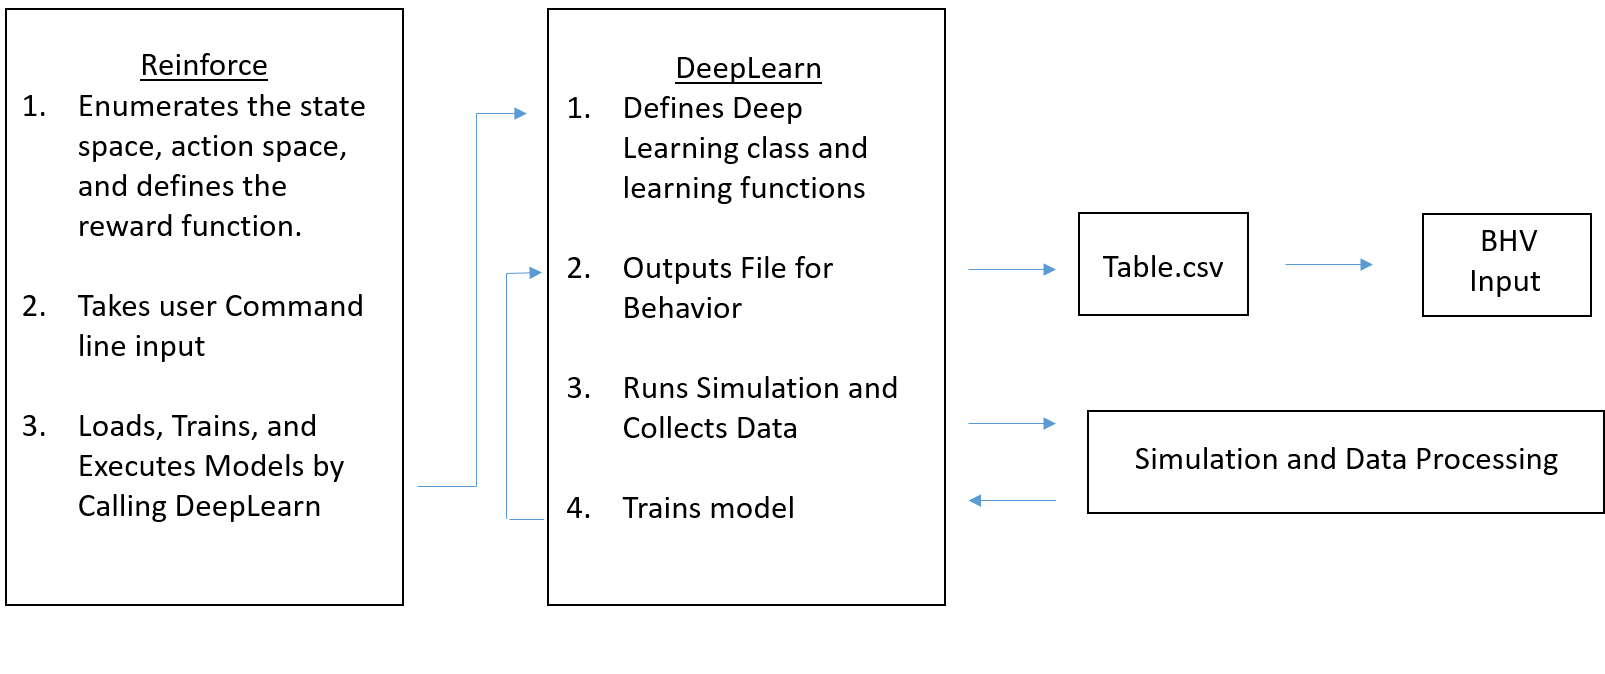
\includegraphics[width=0.8\textwidth]{../images/LearningInteractionDiagram.png}
	\caption{{\bf Learning Script File Interaction Diagram} }
	\label{fig_learn_diagram}
\end{figure}

\subsection{Scripts for Running Simulations}
\begin{description}
	\item[Tester.sh] - Runs the simulation for a set amount of time and then kills it. It then extracts notifications from \mvar{INP\_STAT} in the relevant \texttt{MOOSLogs} to get raw state and action information and writes the resulting \texttt{.csv} to the \texttt{results} directory.
	
	\item[launch\_reinforce.sh] - Launches the simulation with Felix on the red team exhibiting the learned. behavior.
	
	\item[run.sh] - A simple script to run a simulation with the current model and \app{pMarineViewer} running.	
\end{description}  


\subsection{Scripts for Parsing Simulation Data}
\begin{description}
	\item[log\_converter.py] - Extracts important information from files in the \texttt{results} directory and writes it to a new file in the \texttt{processed} directory. (these can be changed in the \texttt{Constants.py} file to be different directories).
\end{description}

\begin{figure}[H]
	\centering 
	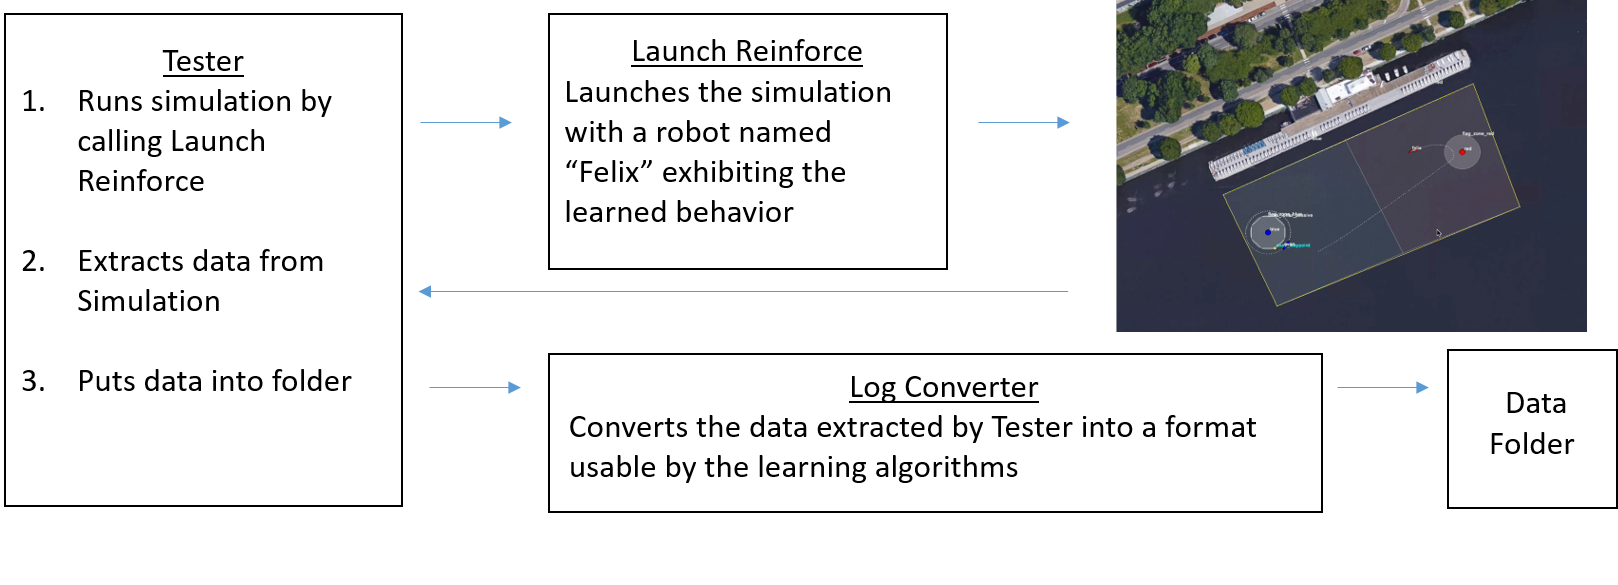
\includegraphics[width=0.7\textwidth]{../images/SimulationInteractionDiagram.png}
	\caption{{\bf Simulation and Data Processing File Interaction Diagram}}.
	\label{fig_sim_diagram}
\end{figure}

\vspace{0.1in}


%======================================================================
\section{Types of Learning Algorithms Available}
%======================================================================

\subsection{Fitted Q Learning}
The algorithm makes one neural net per action, each of which takes in a state as input and outputs the predicted reward of doing that action at that state. The goal is to correctly approximate the Q-Value function which maps state, action pairs to their expected reward. Once trained, the robot acts by choosing the action for which the expected reward is greatest given the state that it is currently in. The mechanics of building the neural neat and training it are provided by the \texttt{Keras} Python library.

\begin{figure}[H]
	\centering 
	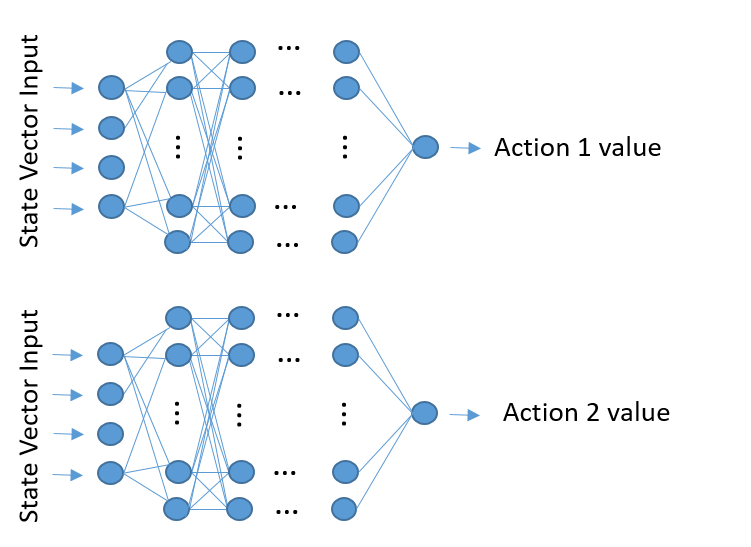
\includegraphics[width=0.7\textwidth]{../images/fittedNet.png}
	\caption{{\bf Fitted Neural Net Structure:} Seperate neural nets for each action. They all take in the same state vector as input, and we select the action which has the neural net with the highest output for that state vector.}
	\label{fig_fitted_net}
\end{figure}

\vspace{0.15in}
\begin{listing}{Basic Algorithm for Fitted Q Learning}
	\label{basic_fitted_alg}
	\footnotesize
	\begin{verbatim}
	1  =============================================================== 
	2  Fitted Q Learning Algorithm PseudoCode                   
	3  =============================================================== 
	4                                                                  
	5  initialize model_NN_dict
	6  initialize target_NN_dict
	7  
	9  //setup the neural nets
	8  for action in actionspace:
	9       model_NN_dict[action] <- new neural net with 1 output node
	11      target_NN_dict[action] <- new neural net with 1 output node
	12	
	13 //get data and train neural nets
	14 for iters <- 0 ; iters < total_iterations:
	15      data <- data from running a simulation with model 
	16      store data into memory
	17      training_set <- Random sample of experiences from memory
	18
	19      for experience in training_set: 
	20          expected <- Caculated expected reward for experience based on target_NN
	16          //seperate experience into its state, action, nextstate, reward pairs
	17          (state, action, newstate, reward) <- experience
	18          train model_NN_dict[action] on state input to target output "expected"
	22 
	23      //update target network
	24      target_NN_dict <- model_NN_dict

	\end{verbatim}
	\normalsize
\end{listing}


\subsection{Deep Q Learning (DQN)}
The algorithm makes one neural net that takes in a state representation as input and outputs the expected reward for each possible action. The neural net has one output node for each possible action in the action space. Then, like with Fitted Q Learning, the algorithm acts by picking the action with the maximum expected reward. The benefits of DQN over the fitted algorithm is that it is faster to train due to the fact that it has a single neural net instead of multiple and when it learns the weights for the correct output for one action for some state, it may help in learning the correct weights for other actions for that state. However, it also has less expressibility in terms of how complex a function it can approximate, since all but the last layer of the neural network have shared weights for all the actions.

\begin{figure}[H]
	\centering 
	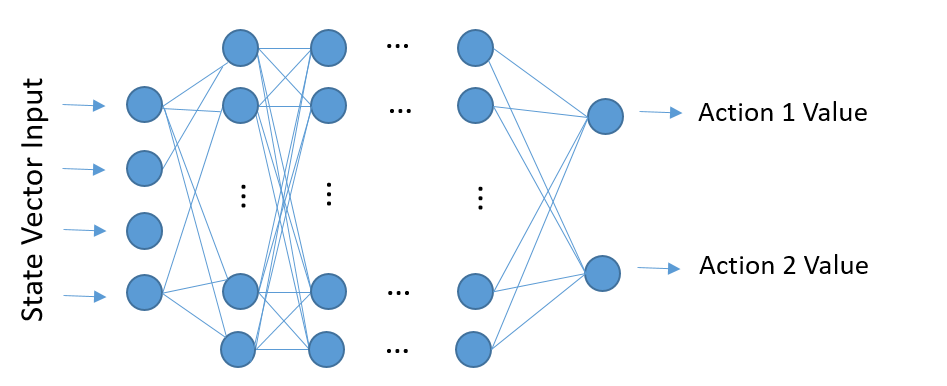
\includegraphics[width=0.7\textwidth]{../images/deepQNet.png}
	\caption{{\bf Deep Q Neural Net Structure:} One neural net for all the actions, with one output per action. Takes in a state vector as input, and we select the action which has the highest output from the neural net.}
	\label{fig_deep_q_net}
\end{figure}

\vspace{0.15in}
\begin{listing}{Basic Algorithm for Deep Q Learning}
	\label{lst_uSpeechRec_econfig}
	\footnotesize
	\begin{verbatim}
	1  =============================================================== 
	2  Deep Q Learning Algorithm PseudoCode                   
	3  =============================================================== 
	4                                                                  
	5  initialize model_NN <- new neural net with 1 output node per action
	6  initialize target_NN <- new nueral net with 1 output node per action
	7	
	8  //get data and train neural nets
	9  for iters <- 0 ; iters < total_iterations:
	10      data <- data from running a simulation with model 
	11      store data into memory
	12      training_set <- Random sample of experiences from memory
	13
	14      for experience in training_set: 
	15          expected <- Caculated expected reward for experience based on target_NN
	16          //seperate experience into its state, action, nextstate, reward pairs
	17          (state, action, newstate, reward) <- experience
	18          train model_NN on state input to target output "expected"
	19 
	20      //update target network
	21      target_NN <- model_NN   
	                                                     
	\end{verbatim}
	\normalsize
\end{listing}


%======================================================================
\section{Making A Model}
%======================================================================

Change the \texttt{user\_path} variable to the path to your moos-ivp-argupta tree. Change the parameters in \texttt{Constants.py} to form the model as desired. More specifics on the parameters in \texttt{Constants.py} are below. Once the parameters are set, the model is ready to be trained. 

\subsection{Constants.py}
\texttt{Constants.py} contains all the important information for the training and testing algorithms and is the primary file that needs to be edited to customize the machine learning model. Before editing any other portions of \texttt{Constants.py}, change the \texttt{user\_path} variable to the path to your \texttt{moos-ivp-argupta} tree. \texttt{Constants.py} has four main sections listed below.

\subsubsection{State Definition}
The state class is a way of holding all the state information together. It has the fields:
\begin{description}
	\item[Index] location of this parameter in the input vector.
	
	\item[Type] the type of information the state contains. This can be either 
	\texttt{"binary"}, \texttt{"distance"}, \texttt{"angle"}, or \texttt{"raw"}. \texttt{"Binary"} type states can only be $0$ or $1$. \texttt{"Distance"} type states represent the distance between \texttt{vehicle} (defined below) and the robot running the learned behavior. \texttt{"Angle"} type states represent the angle betwwn \texttt{vehicle} and the robot running the learned behavior. Finally, \texttt{"raw"} type states represent raw values. These specifications are used by \app{BHV\_Input} to insert the correct type of value into the state vector. 
	
	\item[Normalized]  A boolean flag of whether or not to scale the variable to be between $0$ and $1$ (based on the range parameter). It is recommended that it be set to true for better neural net performance.
	
	\item[Range] A tuple that is used for variables that are not of type \texttt{"binary"}. Sets the minimum and maximum value that this variable can have and is used to standardize the variable between $0$ and $1$ if the \texttt{standardized} flag is set to \texttt{true}. 
	
	\item[Vehicle] the vehicle who's info we are using. This is used when finding the distance or the angle to another vehicle. Set this parameter to the name of the vehicle whose distance or angle is desired, and set \texttt{var} to \texttt{"player"}. The default value is \texttt{"self"}.
	
	\item[Var] The variable which is providing the information. Can be any of the following:
	\begin{description}
		\item[flag] can be used to get the distance or angle from the vehicle to the flag. Needs to define \texttt{var\_mod} as either \texttt{"self"} (for own flag) or \texttt{"enemy"} (for enemy flag).
		\item[team] binary variable that is $1$ if blue team and $0$ if red team. 
		\item[tagged] binary variable that is $1$ if the vehicle is tagged and $0$ if not tagged.
		\item[has\_flag] binary variable that is $1$ if enemy flag captured and $0$ otherwise.
		\item[player] used when vehicle is not \texttt{self}. Returns the distance or angle (as specified in type) from the vehicle to the robot running the machine learning model.
		\item[x/y/heading] these can be used with \texttt{"raw"} state parameters. They will provide the raw. \texttt{x} coordinate, \texttt{y} coordinate, or \texttt{heading} of the vehicle. 
	\end{description}
	\item[var\_mod] Additional variable information such as \texttt{"self"} or \texttt{"enemy"} which are used for deciding which flag to use if asking for flag info. 
	\item[bucket] The size chunks that this variable is discretized into. Set to $1$ as default (not discretized).
	
\end{description}
\texttt{Constants.py} creates a dictionary (hashmap) called \texttt{state} which contains all the definitions for different parts of the state vector for easy access. These definitions are automatically passed to all the other files, including \texttt{BHV\_Input}, to make the correct state definition and pass it through the files automatically. 

\subsubsection{Hyper Parameters}
The second section of \texttt{Constants.py} contains the terms that control how the neural net is structured, and how it is trained. These parameters are important for making a neural net that is capable of approximating the Q-value accurately, as well as deciding how the neural net is trained.

\begin{description}
	\item[num\_layers] The number of layers in the neural network.
	\item[num\_units] number of units per layer in network.
	\item[num\_traj] number of times a simulation is run per iteration to make dataset.
	\item[iters] number of iterations for training (can be arbitrarily high since model is saved on each iteration and training can be stopped any time).
	\item[lr] learning rate for the Adam Optimizer used to train the neural net.
	\item[training\_type] whether trained with \texttt{"stochastic"} gradient descent or \texttt{"batch"} gradient descent.
	\item[eps\_min] the minimum rate at which actions are picked at random (exploration).
	\item[eps\_init] the starting rate ar which actions are picked at random.
	\item[eps\_decay] the rate at which the randomness of actions diminishes per iteration.
	\item[epochs] how many times the the optimizer is run on a batch of training data.
	\item[batch\_size] the number of examples randomly picked from memory when training.
	\item[batches\_per\_training] the number of times we pick out and train on batch of size \texttt{batch\_size} per iteration.
	\item[alg\_type] selects which algorithm to use, can be either \texttt{"DQL"} or \texttt{"fitted"}.
\end{description}
\subsubsection{pLearn Parameters}
These are parameters that are used in the reward function and learning functions, define the action space that the robot uses, and decide how often to save snapshots of the model.
\begin{description}
	\item[speeds] possible speeds that the action can have.
	
	\item[relative] switch to actions that add or subtract from heading rather than set an absolute heading to take. In practice, absolute headings tend to work better. 
	
	\item[rel\_headings] possible headings for relative actions (only relevant if \texttt{relative} is \texttt{true}).
	
	\item[thets\_size\_act] the block size for how spaced out the possible thetas are in the action space.
	
	\item[discount\_factor] the rate at which future rewards are discounted (each timestep ahead that a reward is, it gets multiplied by the discount factor).
	
	\item[max\_reward] the maximum reward possible at the goal state.
	
	\item[neg\_reward] the negative reward used as punishment for bad actions (such as going ouut of bounds or getting tagged).
	
	\item[reward\_dropoff] the rate at which reward diminishes as you move away from the goal.
	
	\item[max\_reward\_radius] the radius around the goal that has \texttt{max\_reward}.
	
	\item[save\_iteration] boolean for whether to have the model automatically save checkpoints every \texttt{save\_iter\_num} iterations. 
	
	\item[save\_iter\_num] how often the model is saved.
	
	\item[players] a list of the other players in the simulation. Allows 
	\texttt{BHV\_Input} to keep track of them. 
	
	\item[mem\_type] whether the memory is a \texttt{"set"}, a \texttt{"deque"}, or a \texttt{"memory per action"}. A set makes an unbounded memory with no repeating experiences. A deque makes a memory of fixed length (\texttt{self.mem\_length}) that may have multiple of the same experiences, but keeps track of more recent experiences. Memory per action makes a seperate deque for each action with fixed length (\texttt{self.mem\_length}), and samples are taken equally from each action deque.
	
	\item[mem\_length] the length of the memory if using \texttt{"deque"} memory type.
	
	\item[mem\_thresh] the threshold at which the program goes from sampling one batch per iteration to sampling \texttt{batches\_per\_training} batches per iteration.
	
	\item[end\_at\_tagged] boolean that dictates whether tagged states count as terminal states (i.e. there are no transitions recorded that go from a tagged state to another state).
	
	\item[num\_test\_iters] The number of simulations the test script runs per model in the testing directory.
	
\end{description}

\subsubsection{File Paths}
The last section of \texttt{Constants.py} defines the system paths to all the important files that are being used by the learning algorithms. These parameters need to be edited whenever a new model is created, or a model is loaded. More specific documentation is available in the \texttt{Constants.py} file. 
\begin{description}
	\item[sim\_cmd] path to the simulation running command.
	
	\item[process\_path] path to folder to get the data to be processed.
	
	\item[process\_cmd] path to script to process the raw data at \texttt{process\_path}.
	
	\item[read\_path] path to the processed data folder.
	
	\item[out\_address] path to where \texttt{table.csv} should be output so that it can be read by \texttt{BHV\_Input}. This should be the path to the folder containing the \texttt{.bhv} file running \texttt{BHV\_input}.
	
	\item[load\_model\_dir] path to the folder where an existing model should be loaded from.
	
	\item[save\_model\_dir] path the folder where we should save the model that is being trained.
	
	\item[mem\_address] path to the folder where a \texttt{memory.txt} file is so that we can load it into the program. Make sure that the memory file has the same state and action definitions as the current model. If no such file, leave the address as an empty string.
	
	\item[test\_address] path to the folder holding the models that need to be tested (with sub folders labeled \texttt{iteration\_\#}).
\end{description}

\subsection{Defining the Reward Function}
The reward function is defined in \texttt{reinforce.py}. As is, it checks whether the robot is tagged, and gives it a negative reward if that is the case. Otherwise it gives the robot a reward proportional to its distance away from the enemy flag. If these parameters no longer exist in \texttt{Constants.state} or a new reward function is needed, just redefine the function in \texttt{reinforce.py} as desired.

\subsection{Modifying the Simulation Scripts}
\subsubsection{Changing the Time For the Simulation}
In \texttt{Tester.sh}, edit the \texttt{while} loop to change the counts for how many times the while loop sleeps before killing the simulation. To change the time warp edit the number next to the \texttt{./launch\_reinforce.sh} command. 

\subsubsection{Editing the Simulation}
Edit files in the \texttt{simulation\_engine/} folder as needed to edit the nature of the simulation. To edit the simulation run by the training scripts, edit \texttt{launch\_reinforce.sh}. To add more players to the game, add the appropriate m200 \texttt{launch\_*} script and set a robot name not yet selected and the team that you would like the robot to be on. To remove a player, just delete or comment out the line with its launch script in \texttt{launch\_reinforce.sh}. 

\end{document}

